\chapter{IMPLEMENTATION}
\label{ch:lex_yacc}


The architecture demonstrated in the Fig 1 with the main functionalities include sending the emails and tracking the bounces. Initially, all the data sent to the lambda using the API gateway which handles the request and response for the whole operation. Upon reaching the lambda, JavaScript Object Notation (JSON) objects from the string parameters preprocessed, the html part of the email along with the subject made into SES templates accessed by other lambdas and the emails batched no more than 50 emails per batch and placed in a Simple queue Service[5] queue. The ordering of the messages is important hence, we use a First In First Out queue, which triggers another lambda that sends emails to all the 50 recipients using a templated email function by accessing the template that we created earlier. We set a flag to mark the end of the batches deleting the template by the end of the execution.


\section{Frontend}

The web application is used to fill and send the emails to all the users at the same time. The application is built using ReactJS library and bootstrap library to style the web page. A basic layand intuitive layout is given considering the web application is mostly used as internal software within an organization or various organizations as a service. 
The fields that need to be filled are

\begin{enumerate}
	\item \textbf{Emails} - Comma seperated values of the emails with spaces and that follows the standard email format.  
	\item \textbf{Names} - Comma separated values of the names corresponding to the emails above it is not a required field. The names will be made into empty strings in the preprocessing.
	\item \textbf{Subject} - String value giving the subject. It is a mandatory field.
	\item \textbf{html} - The email body that is sent to the users. It is interpreted as html code when sent to the lambda function.
	\item \textbf{Sender's email} - The senders email needs to be verified by OTP with AWS console before sending the emails. After an email is verified it is added into the dropdown by the admin. Any one of the verified emails can be used.
\end{enumerate}


\begin{figure}[H]
            \centering
            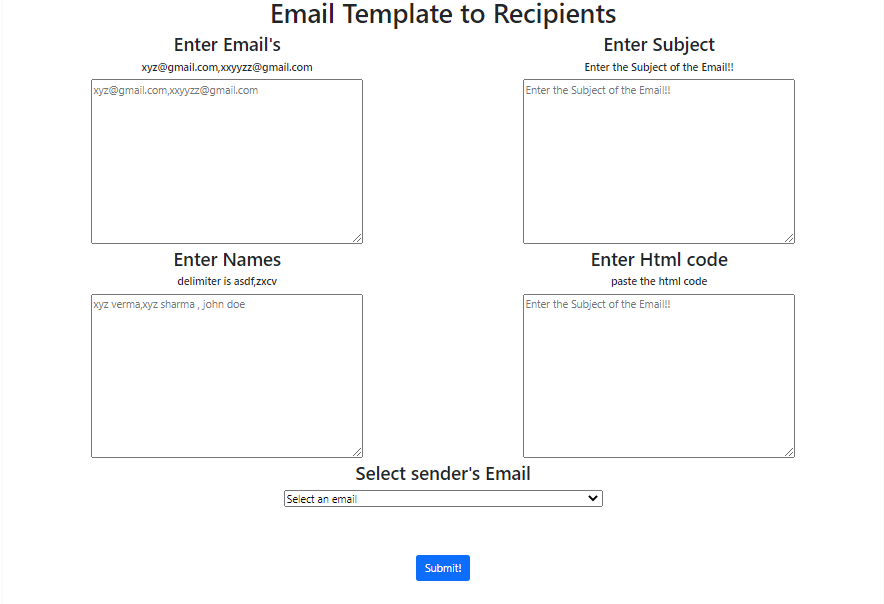
\includegraphics[width=150mm,height=90mm]{figures/frontend_1.png}
            \caption{Frontend Web Application}
            \label{fig:frontend-web}
\end{figure}

In Figure \ref{fig:frontend-web} The web application made using the styling packages is shown. All the respective fields that were mentioned before can be filled out by the user and click on submit to initialize the preprocessing and sending of data to the serverless functions.


\begin{figure}[H]
            \centering
            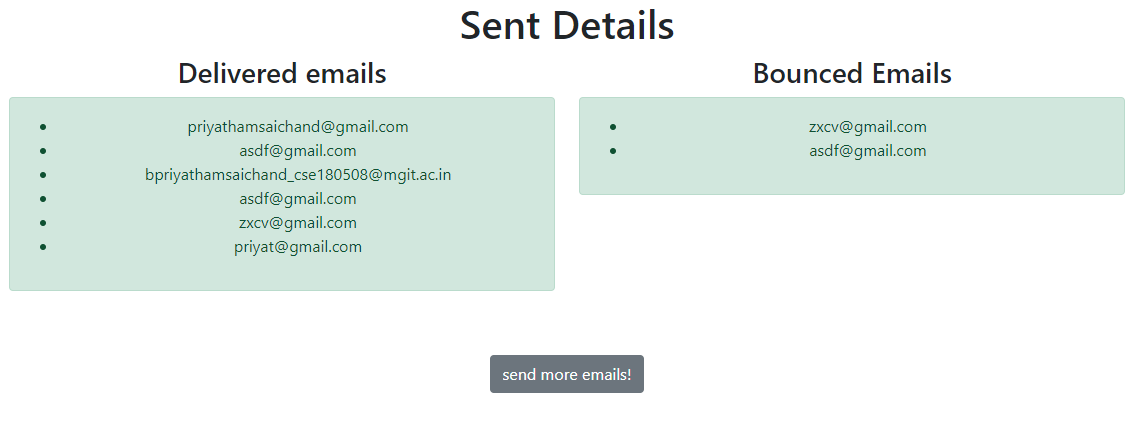
\includegraphics[width=130mm,height=90mm]{figures/result_1.png}
            \caption{Output webpage}
            \label{fig:frontend-output}
\end{figure}


In Figure \ref{fig:frontend-output} The output webpage that is returned after the emails are sent is shown.  

\section{Serverless Functions}
To implement the business logic that is present in the backend. Four lambda functions where created to be used to send and manage the bounces that are generated. Their functionalities are described as follows.

\subsection{email\_batcher}

The purpose of this function is to receive the POST request payload with all the required information such as emails, names, sender's email and subject. It creates the email template with the HTML and sender's email. As per the constraints mentioned in design and methodology, upto 50 emails are batched into a single JSON object and sent into the FIFO queue. All the preprocessing of the string data to json objects is done in this function and is the first function executed with every API call. This lambda function is invoked as a trigger with API gateway used to handle the API endpoints of the application. 


\subsection{sqs\_mailer}

This function is used to send the emails obtained from the FIFO queue. It uses the template that was created by email\_batcher and uses the SES service to send the emails to 50 email addresses along with their names using the sender's email addresses provided. It is triggered by the message in the queue and it can be scaled to meet the number of messages that are available in the queue. Same instance of the lambda function can be used after it is executed or seperate instances can be used based on the concurrency limit given to the lambda function which is 100 in this case.

\subsection{bounce\_mailer}

After the emails are sent, The bounces are sent to the SNS service that triggers this function to collect and filter the json object that is provided and send the bounced email, timestamp to the Dynamo DB for every bounce that occurs. 
 

\subsection{bounce\_db}

Upon successful sending and return of the email\_batcher function the application requests to get all the bounce emails that were accumulated in the database at the given moment using the timestamp and obtained bounce emails as a response to the POST request it sends using another API endpoint. After the bounced emails are retrieved from the database and stored in a JSON object they are cleared from the Database. For next bulk email sending.  


\section{API endpoints}
\label{api_endpoint}

In this section, we will discuss the details on how the REST API calls are made to the serverless backend and the endpoints that are used along with how the request and responses of the endpoints are configured. Two endpoints were used which are as follows 


\subsection{Email sending}
We use an API gateway REST API that is connected to the lambda function of email\_batcher. Thunderclient API testing extension is used with Visual Studio Code to test the API capabilities.
The url of the endpoint is given by 
\url{https://slb37ny1bh.execute-api.ap-south-1.amazonaws.com/prod/email\_batcher}.\par
The emails parameter is used to send the array of emails seperated by commas. The names parameter follows the same schema and the name of the person corresponds to the email provided and all the email addresses without a name at the end are defaulted to empty strings in the preprocessing of the Javascript Application.

\begin{figure}[H]
            \centering
            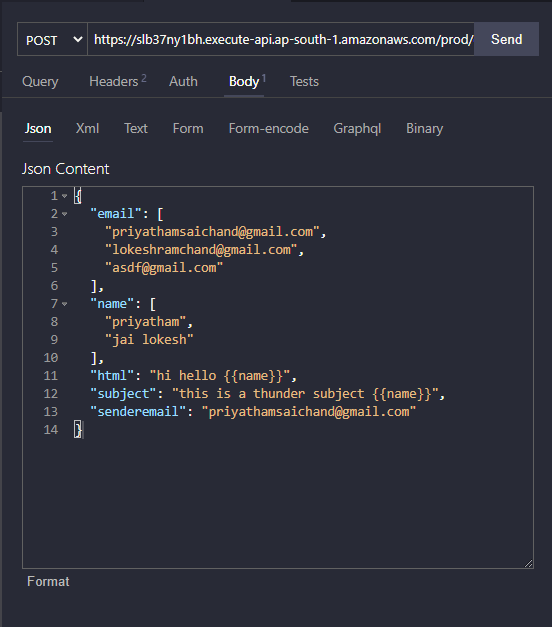
\includegraphics[width=150mm,height=82mm]{figures/api_1.png}
            \caption{Email sending API request}
            \label{fig:email-api}
\end{figure}



In fig \ref{fig:email-api} we show the schema of the request API and all the parameters that needs to be sent. 
\subsection{bounce sending}
We use this API to request the server for the bounce email records that were placed in Dynamo DB.We send a POST request with null parameters and receive the bounce emails. The API end point is given by.

\url{https://slb37ny1bh.execute-api.ap-south-1.amazonaws.com/prod/bounce\_db}

The emails are returned in the form of array of emails and timestamps. Once the bounced emails arrive the delivered emails are computed using the sent emails from the sent email data and the difference of sent and bounced emails gives rise to delivered emails.



